%% For double-blind review submission, w/o CCS and ACM Reference (max submission space)
\documentclass[sigplan,9pt,review,anonymous]{acmart}\settopmatter{printfolios=true,printccs=false,printacmref=false}
%% For double-blind review submission, w/ CCS and ACM Reference
%\documentclass[sigplan,10pt,review,anonymous]{acmart}\settopmatter{printfolios=true}
%% For single-blind review submission, w/o CCS and ACM Reference (max submission space)
%\documentclass[sigplan,10pt,review]{acmart}\settopmatter{printfolios=true,printccs=false,printacmref=false}
%% For single-blind review submission, w/ CCS and ACM Reference
%\documentclass[sigplan,10pt,review]{acmart}\settopmatter{printfolios=true}
%% For final camera-ready submission, w/ required CCS and ACM Reference
%\documentclass[sigplan,10pt]{acmart}\settopmatter{}


%% Conference information
%% Supplied to authors by publisher for camera-ready submission;
%% use defaults for review submission.
\acmConference[LICS'18]{Logic in Computer Science}{July 09--12, 2018}{Oxford, UK}
\acmYear{2018}
\acmISBN{} % \acmISBN{978-x-xxxx-xxxx-x/YY/MM}
\acmDOI{} % \acmDOI{10.1145/nnnnnnn.nnnnnnn}
\startPage{1}

%% Copyright information
%% Supplied to authors (based on authors' rights management selection;
%% see authors.acm.org) by publisher for camera-ready submission;
%% use 'none' for review submission.
\setcopyright{none}
%\setcopyright{acmcopyright}
%\setcopyright{acmlicensed}
%\setcopyright{rightsretained}
%\copyrightyear{2017}           %% If different from \acmYear

%% Bibliography style
\bibliographystyle{ACM-Reference-Format}
%% Citation style
%\citestyle{acmauthoryear}  %% For author/year citations
%\citestyle{acmnumeric}     %% For numeric citations
%\setcitestyle{nosort}      %% With 'acmnumeric', to disable automatic
                            %% sorting of references within a single citation;
                            %% e.g., \cite{Smith99,Carpenter05,Baker12}
                            %% rendered as [14,5,2] rather than [2,5,14].
%\setcitesyle{nocompress}   %% With 'acmnumeric', to disable automatic
                            %% compression of sequential references within a
                            %% single citation;
                            %% e.g., \cite{Baker12,Baker14,Baker16}
                            %% rendered as [2,3,4] rather than [2-4].


%%%%%%%%%%%%%%%%%%%%%%%%%%%%%%%%%%%%%%%%%%%%%%%%%%%%%%%%%%%%%%%%%%%%%%
%% Note: Authors migrating a paper from traditional SIGPLAN
%% proceedings format to PACMPL format must update the
%% '\documentclass' and topmatter commands above; see
%% 'acmart-pacmpl-template.tex'.
%%%%%%%%%%%%%%%%%%%%%%%%%%%%%%%%%%%%%%%%%%%%%%%%%%%%%%%%%%%%%%%%%%%%%%


%% Some recommended packages.
\usepackage{tikz}
\usetikzlibrary{positioning}
\usepackage{stmaryrd}
\usepackage{multicol}
\usepackage{booktabs}   %% For formal tables:
                        %% http://ctan.org/pkg/booktabs
\usepackage{subcaption} %% For complex figures with subfigures/subcaptions
                        %% http://ctan.org/pkg/subcaption
\newcommand{\maps}{\colon}
\newcommand{\into}{\hookrightarrow}
\newcommand{\interp}[1]{\llbracket #1 \rrbracket}

\begin{document}

%% Title information
\title{Logic as a distributive law}         %% [Short Title] is optional;
                                        %% when present, will be used in
                                        %% header instead of Full Title.
%\titlenote{with title note}             %% \titlenote is optional;
                                        %% can be repeated if necessary;
                                        %% contents suppressed with 'anonymous'
%\subtitle{Subtitle}                     %% \subtitle is optional
%\subtitlenote{with subtitle note}       %% \subtitlenote is optional;
                                        %% can be repeated if necessary;
                                        %% contents suppressed with 'anonymous'


%% Author information
%% Contents and number of authors suppressed with 'anonymous'.
%% Each author should be introduced by \author, followed by
%% \authornote (optional), \orcid (optional), \affiliation, and
%% \email.
%% An author may have multiple affiliations and/or emails; repeat the
%% appropriate command.
%% Many elements are not rendered, but should be provided for metadata
%% extraction tools.

%% Author with single affiliation.
\author{Gregory Meredith}
%\authornote{with author1 note}          %% \authornote is optional;
                                        %% can be repeated if necessary
%\orcid{nnnn-nnnn-nnnn-nnnn}             %% \orcid is optional
\affiliation{
  \position{President}
%  \department{Department1}              %% \department is recommended
  \institution{RChain Cooperative}            %% \institution is required
%  \streetaddress{Street1 Address1}
  \city{Seattle}
  \state{WA}
%  \postcode{Post-Code1}
  \country{USA}                    %% \country is recommended
}
\email{lgreg.meredith@gmail.com}          %% \email is recommended

%% Author with two affiliations and emails.
\author{Michael Stay}
%%\authornote{with author2 note}          %% \authornote is optional;
                                        %% can be repeated if necessary
%%\orcid{nnnn-nnnn-nnnn-nnnn}             %% \orcid is optional
\affiliation{
  \position{Cofounder and CTO}
%%  \department{Department2a}             %% \department is recommended
  \institution{Pyrofex Corporation}           %% \institution is required
%%  \streetaddress{Street2a Address2a}
  \city{Orem}
  \state{UT}
%%  \postcode{Post-Code2a}
  \country{USA}                   %% \country is recommended
}
\email{stay@pyrofex.net}         %% \email is recommended


%% Abstract
%% Note: \begin{abstract}...\end{abstract} environment must come
%% before \maketitle command
\begin{abstract}
The internal logic of a category interprets objects as collections, morphisms as terms with one free variable, and subobjects as predicates.  We describe a related but different approach to realizability of types.  We use two monads; the first monad $T$ describes the terms of a programming language, while the second monad $C$ describes a notion of collection.  Formulae are terms in $T+C$ while realizations are terms in $CT.$  Realization is a natural transformation defined in terms of the units and joins of the monads as well as a distributive law $\delta\maps TC \Rightarrow CT.$

Finitary monads can capture not only term structure but also reduction relations. When we use such monads in the construction above, the resulting type system is both structural  and behavioral.  Our main result is that the ``arrow'' type constructor in functional programming languages arises as a modality in the structural-behavioral type system.
\end{abstract}


%% 2012 ACM Computing Classification System (CSS) concepts
%% Generate at 'http://dl.acm.org/ccs/ccs.cfm'.
\begin{CCSXML}
<ccs2012>
<concept>
<concept_id>10011007.10011006.10011008</concept_id>
<concept_desc>Software and its engineering~General programming languages</concept_desc>
<concept_significance>500</concept_significance>
</concept>
<concept>
<concept_id>10003456.10003457.10003521.10003525</concept_id>
<concept_desc>Social and professional topics~History of programming languages</concept_desc>
<concept_significance>300</concept_significance>
</concept>
</ccs2012>
\end{CCSXML}

\ccsdesc[500]{Software and its engineering~General programming languages}
\ccsdesc[300]{Social and professional topics~History of programming languages}
%% End of generated code


%% Keywords
%% comma separated list
\keywords{keyword1, keyword2, keyword3}  %% \keywords are mandatory in final camera-ready submission


%% \maketitle
%% Note: \maketitle command must come after title commands, author
%% commands, abstract environment, Computing Classification System
%% environment and commands, and keywords command.
\maketitle

\section{Introduction}

Our paper centers on the insight that both formulae of a structural type system and their realizations can be expressed in terms of a monad $T$ for terms of a programming language and a monad $C$ for collecting the terms.  The realization of a type is the collection of values of that type.  By composing $C$ with $T,$ we get a functor $CT$ for collections of terms.

Structural type systems express types by replacing specific values with a type identifier.  For example, in Facebook's Flow type system for JavaScript, the record
\begin{center}{\tt \{name: "Joe Schmoe", age: 45\}}\end{center}
is a value of type
\begin{center}{\tt \{name: string, age: number\}}.\end{center}
By taking the sum of the monads $T$ and $C,$ we get a monad for structural formulae.

The realization of formulae is given by a natural transformation ${\interp{-}\maps (T+C)\Rightarrow CT,}$ which can be defined in terms of the units and joins of $T, C,$ and a distributive law ${\delta\maps TC \Rightarrow CT.}$  Whenever we can define $T, C,$ and $\delta$ we get a structural type system for the language $T.$

Finitary monads correspond to Lawvere theories.  There is a Lawvere theory for reflexive directed multigraphs that can be extended to describe the graph of terms and rewrites in programming languages without binders like combinator calculi.  Formulae involving edges not only describe structures but also behaviors.

By adding extra syntax for modal operators to $(T+C)$, we can express behavioral types concisely.  The ``possibly'' modality $\diamond t$ denotes the collection of terms that can be rewritten to $t$ in a single step.  Generalizing slightly, we can define a possibility modality that depends on a couple of types $X, Y$ and a two-hole term context $K$: $X\langle K \rangle Y$ denotes the collection of terms $t$ such that there exists a term $u$ of type $X$ and $v$ of type $Y$ such that $K[t, u]$ can rewrite to $v$ in a single step.  In an applicative calculus like the SKI combinator calculus, $X\langle K \rangle Y$ is precisely $X \Rightarrow Y.$

\section{foo}

\if0

\section{Introduction}
Every category has an associated internal logic.  The objects $X$ are interpreted as collections of items of type $X;$ the morphisms $X \to Y$ are interpreted as terms of type $Y$ with a single free variable of type $X.$  Subobjects $P \into X$ are interpreted as predicates $P(X)$ that pick out those items in $X$ for which $P$ is true.

This line of reasoning culminated in the idea of a topos.  The motivating notion of collection in a topos is that of sets, so in any topos we have empty collections, some base collections given by fiat, the ability to form a collection of pairs, a notion of morphism between collections, and a subobject classifier.

In computer programming, we often use collections that have many but not all of these capabilities.  We would like to explore how the internal logic changes with the notion of collection.  Also, types in computer science describe collections of terms of a programming language; we would like these collections to respect the reduction rules of the language.

We can get a structural type system by adding the monad $T$ for the programming language to the monad $C$ for the collection.  The interpretation of these types is given by a natural transformation ${\interp{-}\maps (T+C) \Rightarrow CT}$ defined in terms of the units and joins of $T$ and $C$ and a distributive law ${\delta\maps TC \Rightarrow CT}.$

The monad for the programming language can describe rewrites as easily as terms by making use of the ``edges-only'' presentation of reflexive directed multigraphs.  With edges, a structural type system is also a behavioral type system because we can talk about collections of rewrites.  The ``possibly'' modality $\diamond X,$ for instance, describes a collection of terms that can be rewritten in a single step to terms in the collection $X.$  A generalization of the possibly modality $X\langle K\rangle Y$ describes a collection of terms that when put into a two-hole term context $K$ with a term of type $X$ can be rewritten in a single step to a term of type $Y.$  When we take $K$ to be an applicative context, such terms are usually said to be of type $X \Rightarrow Y.$

\section{Internal logic}

The internal logic of a category views the objects of the category as certain collections, which we will call ``primitive'' to distinguish them from the collections described by $C.$  It is therefore useful to consider what kind of monads we would like to call ``collections''.  At the very least, we would like to be able to add items to the collection and a notion of an empty collection; this requires the algebras of the monad to be monoids.

The microcosm principle \cite{BaezDolan} says, ``Certain algebraic structures can be defined in any category equipped with a categorified version of the same structure.''  For instance, we can only define monoids in monoidal categories, so $C$ and $T$ will necessarily be monads on a monoidal category.  The unit of the tensor product plays a role analogous to the one element set.  We also typically want to apply $T$ to the empty object of generators so that the only built-in terms are the ones from the programming language itself; a mere monoidal category isn't guaranteed to have one of these, but a rig category is.

The free rig category on a category is a 2-monad.  At this point we are actually interested in {\em doctrines}, which are subtly different from 2-monads on Cat \cite{nlabDoctrine}, but those details are outside the scope of this paper.  Each doctrine corresponds to a particular kind of logic: the doctrine of symmetric monoidal categories corresponds to linear logic, the doctrine of Heyting categories corresponds to first-order logic, the doctrine of elementary toposes corresponds to higher-order logic, and so forth \cite{nlabInternalLogicKindsOfInternalLogic}.



\begin{figure}
  \begin{center}
    \begin{itemize}
      \item a generating object $M$
      \item generating morphisms $S,K,I\maps 1\to M$
      \item a generating morphism $(-\;-)\maps M^2 \to M$
      \item a generating 2-morphism $\sigma\maps (((S\;x)\;y)\;z)\Rightarrow ((x\;z)\;(y\;z))$
      \item a generating 2-morphism $\kappa\maps ((K\;x)\;z)\Rightarrow x$
      \item a generating 2-morphism $\iota\maps (I\;z)\Rightarrow z$
    \end{itemize}
  \end{center}
  \caption{A presentation of the Cat-enriched Lawvere theory of the SKI combinator calculus.}
  \label{fig:SKI}
\end{figure}



As computer programmers, we often use abstract data types (ADTs) for describing collections.  The elements of an ADT form a set rather than a category, but we can equip the set with morphisms.  Here we consider defining morphisms from a term $t$ of an ADT to another term $u$ of the ADT to be the inclusions of $t$ as a subterm of $u$ up to relabeling, where by relabeling we mean any data in a production that is not at a recursion point.

The resulting category has two kinds of morphism that interact well: pointwise rewrites of terms in a collection and inclusion of collections into each other.  In most programming languages, there are no equations between rewrites, only equations between structurally equivalent terms.  The result is that $CT\emptyset$ is actually a quiver, the free category on a graph.  Subobjects are isomorphism classes of monos; in a quiver, $g\circ f$ is never equal to $h\circ f$ unless $g=h,$ so all morphisms from rewrites are monos.  The morphisms coming from inclusions are monos by construction.




\section{Comparison with toposes}



\section{Collections}
\section{Formulae}
\section{Realization}
\section{Modalities}
\section{Conclusion}

\begin{enumerate}
  \item \label{topostype:unit} There is a unit type representing the empty collection.
  \item \label{topostype:base} There is a set of base types representing collections granted by fiat.
  \item \label{topostype:product} There are product types representing the special case of using a collection to form pairs and take them apart again.
  \item \label{topostype:function} There are function types representing ways to manipulate collections.
  \item \label{topostype:omega} There is a subobject classifier $\Omega$ representing the collection of ways an element can inhabit a collection.
\end{enumerate}

For an example of point \ref{topostype:product} failing, we may be able to ``pair up'' collections without being able to take them apart again.  If we use the notion of a vector space to collect items rather than a set, then linear transformations are those functions that preserve the structure; the corresponding notion of product is the tensor product, not the cartesian one.  We can take the Kronecker product of a vector in $U$ and a vector in $V$ to get a vector in $U \otimes V,$ but given an arbitrary vector in $U\otimes V,$ there is rarely a way to write it as the Kronecker product of two other vectors.  

More often, it is point \ref{topostype:omega} that fails.  While sets have a clear notion of morphism between them, namely functions, it is not necessarily clear what the appropriate morphism between two lists should be.  A list can be thought of as a linked list, as a free monoid, as a totally ordered multiset, {\em etc.}; each different notion has its own concept of morphism.

  

With this choice, all morphisms are monomorphisms and subobjects correspond to collections over the terminal type.  While the subobject classifier in a topos is isomorphic to collections over the terminal type, the converse does not always hold.

\section{Formulae and realizability}

Types in computer programming describe collections of terms of the programming language.  Often, this is done by allowing type identifiers to appear in place of literals in the grammar.  For instance, in Facebook's Flow type system for JavaScript, we can replace the specific name and age in the record 
\begin{center}
  {\tt \{name: "Joe Schmoe", age: 45\}}
\end{center}
with the types {\tt string} and {\tt number}, respectively, to get a type of records:
\begin{center}
  {\tt \{name: string, age: number\}}.
\end{center}
This suggests that given an ADT $T$ describing terms in a programming language and an ADT $C$ describing a notion of collection, we can sum the two to get an ADT for formulae.  

The interpretation of a formula is a collection of terms.  A collection of terms is simply the composition of the two monads applied to the generators.  Therefore, we expect the interpretation of a formula to be given by a natural transformation
\[ \interp{-}\maps T+C \Rightarrow CT. \]
The natural transformation can be expressed in terms of the units and joins of $T$ together with a distributive law
\[ \delta\maps TC \Rightarrow CT. \]
We think of a collection as a way of ``summing'' terms together and the term constructors themsleves as a kind of formal product.  The distributive law maps products of sums to sums of products.

Such a distributive law may not always exist.  In figures \ref{fig:sets} and \ref{fig:lists}, we show how the ``sets of'' collection monad admits both linear and nonlinear combinators, but the ``lists of'' collection monad only admits linear ones.

\section{Rewrites}
Specifications of programming languages include not only the grammar for the language but also a description of the rewrite rules and the contexts in which the rules apply.  Multisorted Lawvere theories give us a language in which to describe the reflexive graph of terms and rewrites between them.  We have one sort for vertices, one for edges, a pair of function symbols for source and target, and a set of function symbols for generating the specific terms in the grammar and the specific rewrites between terms.  We also have equations for describing structural equivalence.

By referring to edges, formulae can describe behaviors of programs as well as their structure.  Suppose we have a two-hole term context $K$ and we define the type $X\langle K\rangle Y$ to be the set of terms $t$ such that there exist two terms $u\in X$ and $v \in Y$ and a rewrite from $K(t,u)$ to $v.$  In an applicative calculus like lambda calculus or a combinator calculus, we can take the context $K$ to be application; then $X\langle K\rangle Y$ is $X \Rightarrow Y.$  If instead we have a concurrent calculus like pi calculus, we can choose $K$ to be the par operator and $X\langle K\rangle Y$ gives Caires' rely-guarantee modality $X\triangleright Y$.

%% exists_f S⊆VxVxVxE = {r | y <- f(S), r <- y}
%% f(r:V,u:V,v:V,rho:E) = [r] if s(rho) = C(r, u) and t(rho) = v, [] otherwise
%% when C = application, exists_f S has one copy of r for each way to form A => B in S.

\section{Typed terms}
Typing works somewhat differently in this scenario.  Every term is also a formula whose interpretation is the collection containing only that term.  Every term constructor is a type constructor, so we don't immediately get, e.g. that the type of the $K$ combinator is $X \Rightarrow Y \Rightarrow X.$  We have to prove that $K$ satisfies that modality.


\section{Comparison with toposes}

%% types are collections
%% unit type // must have empty collection
%% sorts are types (base collections)
%% product // must be free monoidal
%% internal hom // functions between collections
%% power objects // collections of collections
%% 
%% atomic formulae 
%% base relations A -> P1
%% equality AxA -> P1
%% inhabitation AxPA -> P1
%% 
%% terms
%% *:1, FV(*) = {}
%% const k:A, FV(k) = {}
%% var v:A, FV(v) = {v}
%% fn sym f:A -> B, term t:A => f(t):B, FV(f(t)) = FV(t)
%% s:A, t:B => <s,t>:AxB, FV(<s,t>) = FV(s) ∪ FV(t)
%% s:AxB => left(s):A, FV(left(s)) = FV(s)
%% s:AxB => right(s):B, FV(right(s)) = FV(s)
%% s:B, a:A => λa.s:[A -> B], FV(λa.s) = FV(s) - {a}
%% f:[A->B], t:A => ev(f,t):B, FV(ev(f,t):B) = FV(f) ∪ FV(t)
%% θ:P1, a:A => {a | θ}:P1, FV({a | θ}) = FV(θ) - {a} // special case of λ for B = P1

%% types
%% unit type I
%% sorts are types // sorts here are formulae
%% tensor product
%% internal hom
%% "power" monad P
%% 
%% atomic formulae
%% base relations A -> P1
%% equality A⊗A -> P1 // [] no otherwise yes
%% inhabitation A⊗PA -> P1 // [] no otherwise yes
%% 
%% terms
%% *:1, FV(*) = {}
%% const k:A, FV(k) = {}
%% var v:A, FV(v) = {v}
%% fn sym f:A -> B, term t:A => f(t):B, FV(f(t)) = FV(t)
%% s:A, t:B => <s,t>:A⊗B, FV(<s,t>) = FV(s) + FV(t)
%% s:ΓxA -> B, a:A => λa.s:[A -> B], FV(λa.s) = components(Γ)
%% f:[A->B], t:A => ev(f,t):B, FV(ev(f,t):B) = FV(f) + FV(t)
%% θ:ΓxA -> P1, a:A => {a | θ}:P1, FV({a | θ}) = components(Γ) // special case of λ for B = P1


\begin{figure*}
  \def\w{5}\def\h{2}
  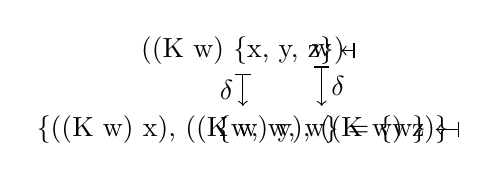
\begin{tikzpicture}
    \node (A) at (0,\h) {((K w) \{x, y, z\})};
    \node (B) at (\w,\h) {w}
      edge [<-|] (A);
    \node (C) at (0,0) {\{((K w) x), ((K w) y), ((K w) z)\}}
      edge [<-|] node [left] {$\delta$} (A);
    \node (D) at (\w,0) {\{w, w, w\} = \{w\}}
      edge [<-|] node [right] {$\delta$} (B)
      edge [<-|] (C);
  \end{tikzpicture}
  \def\w{8}\def\h{2}
  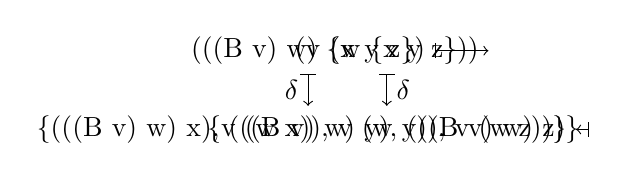
\begin{tikzpicture}
    \node (A) at (0,\h) {(((B v) w) \{x y z\})};
    \node (B) at (\w,\h) {(v (w \{x y z\}))}
      edge [<-|] (A);
    \node (C) at (0,0) {\{(((B v) w) x), (((B v) w) y), (((B v) w) z)\}}
      edge [<-|] node [left] {$\delta$} (A);
    \node (D) at (\w,0) {\{v (w x)), v (w y)), v (w z))\}}
      edge [<-|] node [right] {$\delta$} (B)
      edge [<-|] (C);
  \end{tikzpicture}
\caption{Using the ``sets of'' collection monad with the combinators $K$ and $B$.}
\label{fig:sets}
\end{figure*}




\begin{figure*}
\def\w{5}\def\h{2}
  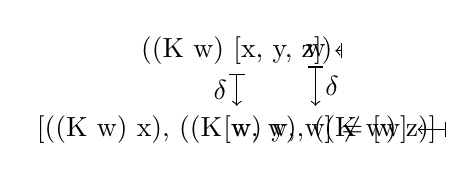
\begin{tikzpicture}
    \node (A) at (0,\h) {((K w) [x, y, z])};
    \node (B) at (\w,\h) {w}
      edge [<-|] (A);
    \node (C) at (0,0) {[((K w) x), ((K w) y), ((K w) z)]}
      edge [<-|] node [left] {$\delta$} (A);
    \node (D) at (\w,0) {[w, w, w] $\ne$ [w]}
      edge [<-|] node [right] {$\delta$} (B)
      edge [<-|] (C);
  \end{tikzpicture}

  \def\w{8}\def\h{2}
  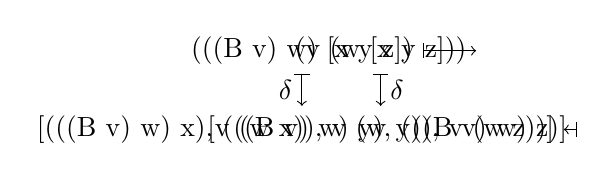
\begin{tikzpicture}
    \node (A) at (0,\h) {(((B v) w) [x y z])};
    \node (B) at (\w,\h) {(v (w [x y z]))}
      edge [<-|] (A);
    \node (C) at (0,0) {[(((B v) w) x), (((B v) w) y), (((B v) w) z)]}
      edge [<-|] node [left] {$\delta$} (A);
    \node (D) at (\w,0) {[v (w x)), v (w y)), v (w z))]}
      edge [<-|] node [right] {$\delta$} (B)
      edge [<-|] (C);
  \end{tikzpicture}
\caption{Using the ``lists of'' collection monad with the combinators $K$ and $B$.  Because $K$ discards information, there is no nontrivial distributive law for the $SKI$ calculus and the list monad.  The $BCI$ calculus, on the other hand, is linear, and works fine with the list monad.}
\label{fig:lists}
\end{figure*}

Given $\delta\maps T+C \Rightarrow CT$ and an algebra $h\maps CTX \to X,$ get algebra $h\delta_X\maps (T+C)X \to X.$


%% ∃_f S = [ y∈Y | ∃x∈X. f(x)=y  ∧  x∈S ] = map f S
%% 
%% f:ℕ->[ℕ]
%% f(x) = [x] if x even, [] otherwise
%% How to write this?
%% x is ``even'' if there exists y st y+y = x
%% 
%% !:X -> 1
%% exists_! S = [•∈1 | ∃x∈X. !(x) = •  ∧  x in S] = S nonempty
%% 
%% S = [x'∈{x} | ∃y∈ℕ. y+y = x' ^ y∈ℕ ]
%% 
%% evens in S⊆ℕ: join [ y∈Y | ∃x:ℕ. f(x) = y  ∧  x ∈ S ] = [y | x <- S, y <- f(x)] = flatmap f S
%% 
%% inhabitation s in S = 1 if not, otherwise yes
%% 
%% ``set-like'' collections: P1 is a classifier 
%% 
\fi

%% Acknowledgments
\begin{acks}                            %% acks environment is optional
                                        %% contents suppressed with 'anonymous'
\end{acks}


%% Bibliography
%\bibliography{bibfile}


%% Appendix
\appendix
\section{Appendix}

Text of appendix \ldots

\end{document}
